\chapter{研究问题的形式化定义}

在本章中,为了后续讨论的方便和统一,我们给出电子表格的编程模型,并解释比如单元格类和单元格缺陷这类核心概念。
为了简化表达,除额外说明之外,我们用\textit{数值单元格}专指那些单元格里的数值是直接给出而不是计算得来的单元格,用\textit{公式单元格}专指那些单元格里的数值是根据自身公式计算得来的单元格。

\section{电子表格的编程模型}

一个电子表格(更准确地说,一个电子表格中的一个工作表)可以被建模成一个集合,其中包含带有表达式的单元格,这些单元格使用二维地址来索引(一个行索引和一个列索引,比如 $B1$ 或者 $C2$)。
数值单元格和公式单元格的表达式分别通过纯粹的数值和公式来刻画。
一个公式通过\textit{单元格引用}来引用另一个单元格,单元格引用也是通过被引用的单元格地址来索引。
用$R$来表示单元格引用的集合,$EXP$来表示表达式的集合,$V$表示纯粹数值的集合。
一个单元格的表达式 $exp$ 要么是一个纯粹数值($v \in V$),一个单元格引用($r \in R$),或者一个引用一个或多个表达式的公式($\varphi $)。
电子表格中使用的函数包括基本的运算符(例如,“+”,“-”,“*”和“/”),以及大量电子表格软件中的内置函数(例如,$SUM$,$AVERAGE$和$MAX$)。
形式化地表达,一个单元格的表达式$exp$为:
\[ exp =\quad v\quad |\quad r\quad |\quad \varphi (exp_1,\dots,exp_n). \]

更进一步,我们定义一个获取引用函数$\sigma(exp)$,该函数返回一个集合,其中包含在一个单元格的表达式中使用到的所有单元格引用。形式化地表达如下:
$$
\sigma(exp) = 
\left\{
    \begin{aligned}
       & \emptyset & exp \in V; \\
       & \{exp\}     & exp \in R; \\
       & \sigma(exp_1) \cup \dots \cup \sigma(exp_n) & exp = \varphi(exp_1, \dots , exp_n).
    \end{aligned}
\right.
$$

\begin{figure}[tp]    
    \centering
    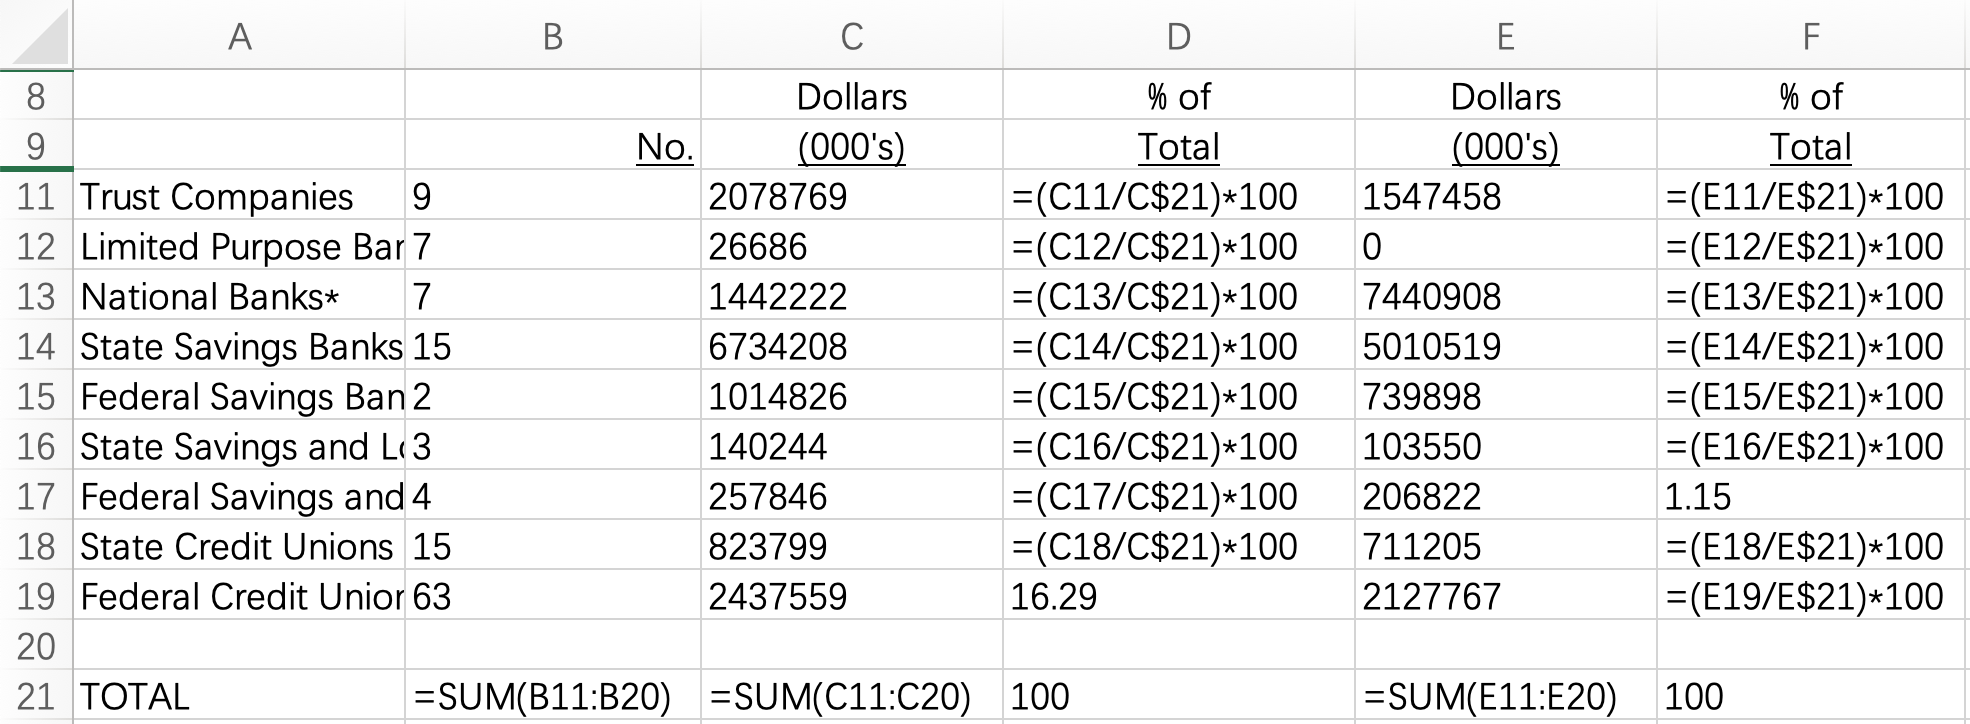
\includegraphics[width=\textwidth]{figure/style-A1.png}
    \caption{截取自EUSES 数据库中的电子表格 summ0602.xls 的工作表summary1201(A1 表示法)}
    \label{figure-A1}
\end{figure}
\begin{figure}[tbp]    
    \centering
    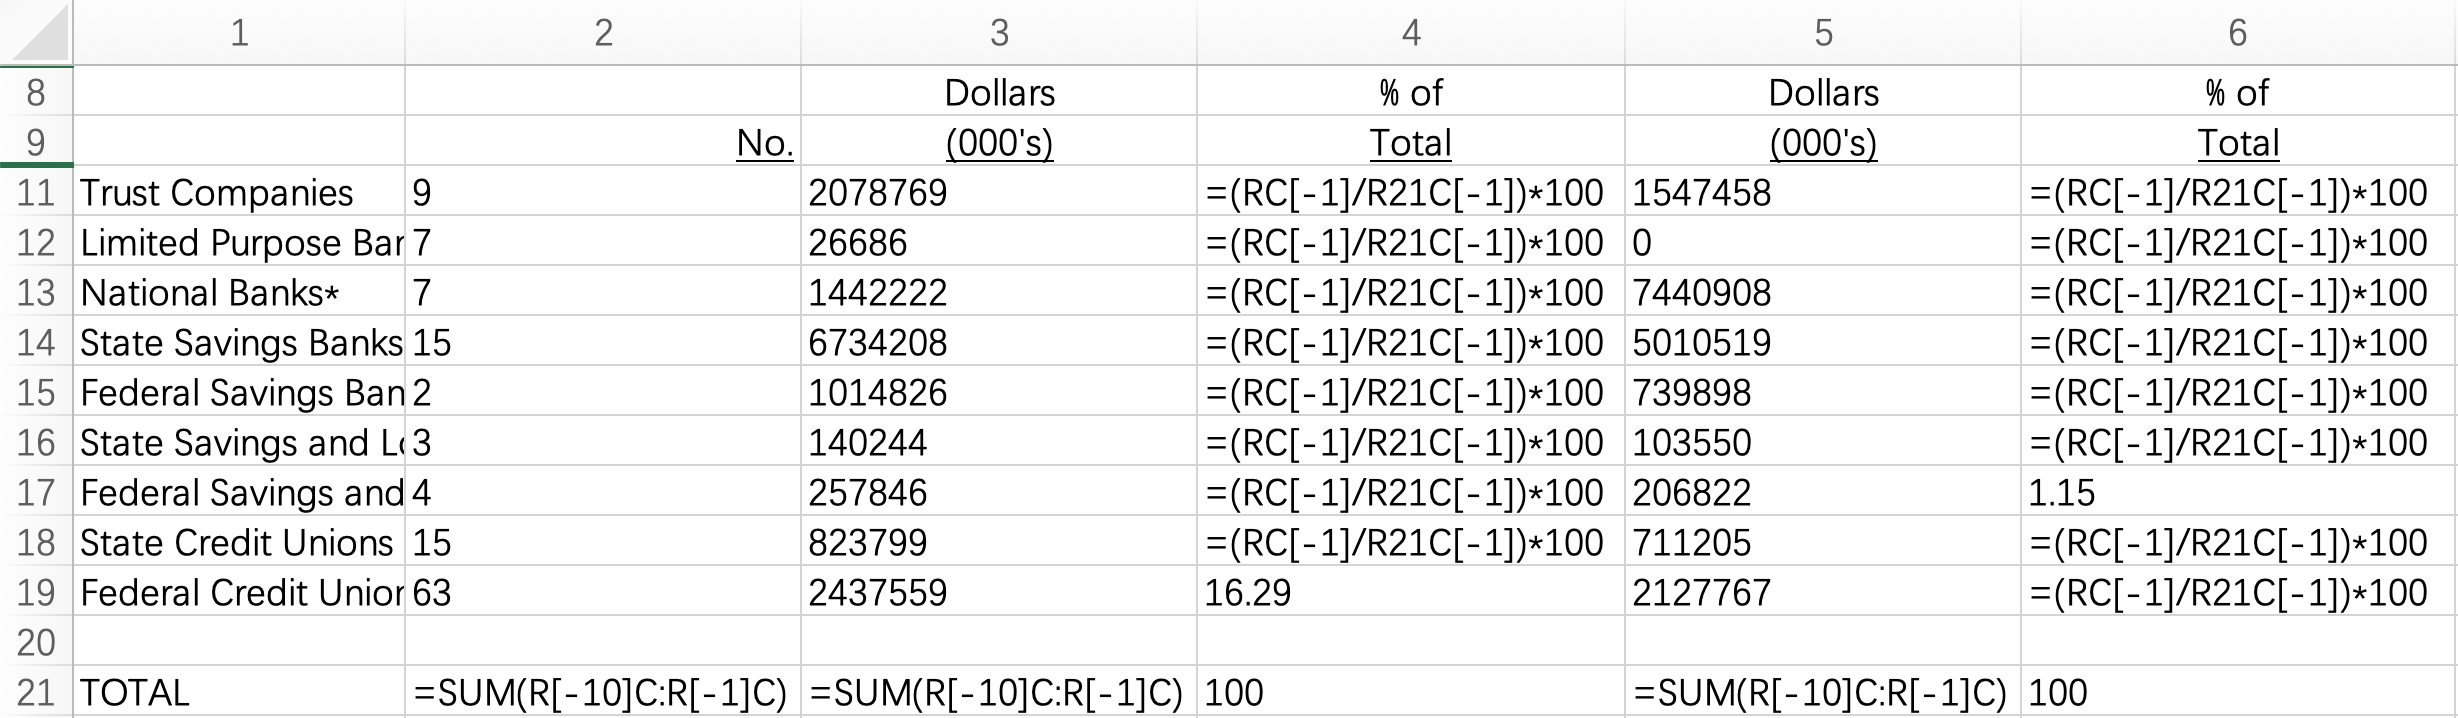
\includegraphics[width=\textwidth]{figure/style-R1C1.png}
    \caption{截取自EUSES 数据库中的电子表格 summ0602.xls 的工作表summary1201(R1C1 表示法)}
    \label{figure-R1C1}
\end{figure}

绝大多数电子表格软件有两种内置的表达公式应用的风格,即\textit{A1表示法} 和 \textit{R1C1表示法} \cite{tan2014bug} ,另一种划分方式是\textit{绝对引用}和\textit{相对引用}。
绝对引用指向特定的单元格,当它在某个表达式中存在,并且该表达式被复制到其他单元格,仍然引用相同的单元格。
相对引用表示单元格地址在当前单元格和被引用单元格之间的偏移量,当该引用被复制到其他单元格时,偏移量保持不变,但实际引用的单元格地址发生了变化。

在 A1 表示法中,一个在第 $X$ 列第 $y$ 行的单元格在相对引用中表示为 $Xy$(例如$B5$),在绝对引用中表示为 $\$X\$y$(例如$\$B\$5$)。
如图\ref{figure-A1}所示,该电子表格使用的是 A1 表示法,且所有单元格引用都是相对引用。

另一方面,在 R1C1表示法中,一个在当前单元格的下方第$n$行和右侧第$m$列的单元格在相对引用中表示为$R[n]C[m]$(其中,$n$($m$)在$n=0$($m=0$)时可以被省略),而一个处在第$n$行,第$m$列的单元格在绝对引用下表示为$RnCm$。
如图\ref{figure-R1C1}所示,该电子表格使用 R1C1表示法,且所有单元格引用都是相对引用。

一个有趣的观察是:含有相似计算模式的公式单元格通常具有语义等价的 R1C1表示的公式形式。
例如,
% 在接下来的讨论中,除额外说明,我们假设表达式$exp$和函数$\sigma(exp)$都使用 R1C1表示法。


\section{单元格类}


\section{公式缺陷}
